\begin{surferPage}[Labs'ın Yedigili]{99 Tekillikli Bir Yedigil}
    Oliver Labs 2004 yılında Mainz Üniversitesinde doktora tezi üstünde çalışırken  derecesi $7$ olan  (yedigil) ve $99$ adet tekilliği olan bir yüzey inşa etti. Bu yedigiller arasında bir dünya rekoru.
Yine de tekillik sayısı $104$'e kadar çıkabilecek bir yüzey var olabilir.
Labs'ın yüzeyi düzgün yedigen simetrisine sahip (soldaki resim).
Yüzeye yukarıdan bakınca bu görülebiliyor  (sağdaki resim):

    \vspace*{-0.3em}
    \begin{center}
      \begin{tabular}{c@{\qquad}c}
        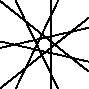
\includegraphics[height=1.5cm]{./../../common/images/labsseptic1.pdf}
        &
        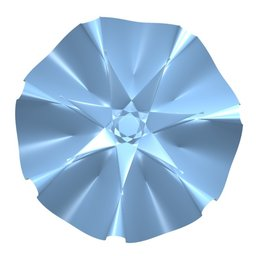
\includegraphics[height=1.5cm]{./../../common/images/labs_septic_von_oben}
      \end{tabular}
    \end{center}
    \vspace*{-0.3em}

Bu yüzeyin inşasında  Oliver Labs bir bilgisayar cebir sistemi olan
    {\sc Singular} (Kaiserslautern Üniversitesi) yazılımını kullandı. Bu yazılım, cebirsel geometri ve tekillik hesaplarında yetkin bir yazılımdır.

Kullandığı temel gözlem, sonlu sayı kümelerinde saymanın doğal bir yolunun olduğuydu. Bunu saatlerden biliyoruz aslında:   saat 24:00, 00:00 demek olduğundan 24:00 $+$ 1 saat  25:00 değil 01:00 olur.
\end{surferPage}
